\documentclass[conference]{IEEEtran}
\usepackage{graphicx}
\usepackage{lipsum}
\usepackage{cite}
% *** MATH PACKAGES ***
\usepackage{amsmath}
% *** SPECIALIZED LIST PACKAGES ***
\usepackage{algorithmic}
% *** ALIGNMENT PACKAGES ***
\usepackage{makecell}
\usepackage{array}
\usepackage{float}
\usepackage[utf8x]{inputenc}

\makeatletter
\def\endthebibliography{%
  \def\@noitemerr{\@latex@warning{Empty `thebibliography' environment}}%
  \endlist
}
\makeatother

\author{
    \IEEEauthorblockN{Shashank Reddy Boosi\IEEEauthorrefmark{1}, David Sison\IEEEauthorrefmark{1}, Harmanpreet Singh\IEEEauthorrefmark{1}, Aravind Murugesan\IEEEauthorrefmark{1}, Allen kombasseril\IEEEauthorrefmark{1}}
    \IEEEauthorblockA{\IEEEauthorrefmark{1} School of Computing\\   { { University of New South Wales}}
    \\\{z5222766, z5019783, z5228917, z5175965, z5232188\}@student.unsw.edu.au}
}

\begin{document}

\title{Computer Vision (COMP9517) Assignment}


% make the title area
\maketitle

% As a general rule, do not put math, special symbols or citations
% in the abstract
\begin{abstract}
 \textbf{\textit{Task 1}} - Diabetic retinopathy, known as diabetic eye disease, is a medical condition which damages the retina due to diabetes mellitus. This report is an attempt to solve the problem where we use Deep Learning to segment the four categories of lesions in a retinal image. We present a network and training strategy that relies on the strong use of data augmentation to use the available annotated samples efficiently. The architecture consists of a contracting path to capture context and a symmetric expanding path that enables precise localization. The model used is a fine tuned U-Net which is an enhanced encoder-decoder CNN model and we attained Jaccard Similarity of 0.3093 and a Dice Similarity of 0.3838 respectively.


\par
\setlength{\parskip}{1em}
\setlength{\parindent}{0em}

\textbf{\textit{Task 2}} - The segmentation of blood vessels can be used for various retinal imaging. We present a report of our study of a Resolution Hierarchy based method. The method reduces computational needs and could detect vessel of different thickness by using a Gaussian resolution hierarchy. The algorithm reported an accuracy of 87.5\% while taking less time to run. 

\paragraph*{Keywords}
Diabetic Retinopathy, Blood Vessels, UNet, Gaussian Pyramid.

\end{abstract}

% no keywords



% For peer review papers, you can put extra information on the cover
% page as needed:
% \ifCLASSOPTIONpeerreview
% \begin{center} \bfseries EDICS Category: 3-BBND \end{center}
% \fi
%
% For peerreview papers, this IEEEtran command inserts a page break and
% creates the second title. It will be ignored for other modes.
\IEEEpeerreviewmaketitle

\section{Task 1}

\subsection{Introduction}
\par
Diabetic retinopathy, a chronic, progressive eye disease, has turned out to be one of the most common causes of vision impairment and blindness especially for working ages in the world today\cite{1}. Retinal abnormal conditions are associated with lesions namely microaneurysms, haemorrhages, hard exudates and soft exudates. The diagnosis in the early stages of the disease is particularly important to receive proper treatment and reduce the chance of progression of the disease to advanced stages which can lead to permanent loss of vision in extreme cases\cite{2}. The presence of these lesions is highly correlated with DR, so detection of their presence is crucial. Retinopathy detection system is usually accomplished by involving a well-trained physician manually detecting vascular abnormalities and structural changes of retina in the retinal fundus images. These results are closely observed by expert readers but they often inconsistent as the method is manual in nature\cite{8}. So an automated method is necessary to identify these defects. 
\par
Most of the problems of computer vision of recent times have been solved with great accuracy with the help of modern deep learning algorithms, Convolutional Neural Networks (CNN's) to name one. Here we are using a tweaked version of the Fully connected convolutional neural network named UNET, which was developed by Olaf Ronneberger et al\cite{unet}, which have shown impressive results for biomedical image segmentation problems with lower number of training images.


Diabetic retinopathy, a chronic, progressive eye disease, has turned out to be one of the most common causes of vision impairment and blindness especially for working ages in the world today\cite{1}.Is is caused by several medical conditions such as prolonged diabetes and ageing. Retinal abnormal conditions are associated with lesions namely microaneurysms, haemorrhages, hard exudates and soft exudates. It is therefore important to identify these defects in a retinal image. The diagnosis in the early stages of the disease is particularly important to receive proper treatment and reduce the chance of progression of the disease to advanced stages which can lead to permanent loss of vision in extreme cases\cite{2}. The presence of these lesions is highly correlated with DR , so detection of their presence is crucial. Retinopathy detection system is usually accomplished by involving a well-trained physician manually detecting vascular abnormalities and structural changes of retina in the retinal fundus images. These results are closely observed by expert readers but they often inconsistent as the method is manual in nature\cite{8}. So an automated method is necessary to identify these defects. Earlier solutions of automated diabetic retinopathy detection system were based on hand-crafted feature extraction and standard machine learning algorithm for prediction\cite{3}. 
\par
Most of the problems of computer vision of recent times have been solved with great accuracy with the help of modern deep learning algorithms, Convolutional Neural Networks (CNNs) to name one. Here we are using a tweaked version of the Fully connected convolutional neural network named UNET, which was developed by Olaf \cite{unet}, which have shown impressive results for Bio medical image semantic segmentation problems with lower number of training images.

\subsection{Related Works}
\par

Automatic diabetic retinopathy detection system can be achieved by various different algorithms and methods. C.Sinthanayothin used Recursive region growing segmentation algorithms along with the use of a new technique , named as Moat Operator to detect defects such as haemorrhages, microaneurysms and hard exudates. they could end up with a sensitivity and specificity for exudate detection of 88.5\% and 99.7\% respectively . They could detect microaneurysms, haemorrhages with a sensitivity and specificity of 88.7\% and 77.5\% respectively. 
\par

Deep learning methods are proven to show good results in image segmentation tasks. Sheikh Muhammad Saiful Islam used Deep learning methods along with data preprocessing and data augmentation for Early Detection and Grading of Diabetic Retinopathy\cite{8}. So, in this work, they have presented a 4 x 4 kernel based CNN network with several preprocessing and augmentation methods to improve the performance of the architecture. their network achieved 98\% sensitivity and more than 94\% specificity in early-stage detection and on the challenging Kaggle EyePACS dataset\cite{9}.
\par
There was also a challenge\cite{idrid} hosted on  Grand Challenges in Biomedical Imaging Platform, which is one of the best platforms for biomedical imaging related competitions. One of the challenges in this competition was mainly to segment the lesions in a retinal image. For lesion segmentation task, most of the participating teams used U-Net architecture\cite{unet}. This network works with very few training images and enables the seamless segmentation of high-resolution images by means of an overlap-tile strategy\cite{idrid}. The best approach for lesion segmentation in this competition used U-Net, with data augmentation boosting results significantly. It resulted in AUC of 0.8263, 0.9716, 0.9540 and 0.9883 for MA, HE, SE and EX respectively. 
\par
Olaf Ronneberger demonstrated the application of the U-NET to three different segmentation tasks\cite{unet}. one of it was a cell segmentation task in light microscopic images. This segmentation task is part of the ISBI cell tracking challenge 2014 and 2015 \cite{6,7}. Here they achieve an average IOU (Intersection over Union) of 92\% .
\par
This motivated us to use U-Net to further modify the network  according to our dataset.

\subsection{Methodology}                                                                     
Fig. \ref{fig:dl} shows us an overview of the methodology pipeline. Our methodology consists of various steps: Image augmentation, Image pre-processing, and Modelling where we start with preparing the dataset, augmenting using selective resampling, preprocessing, fine tuning the model, training and testing. The data-set is taken from IDRiD Grand Challenge \cite{idrid}. We mainly  used imgaug, opencv and pytorch\cite{7} and pandas library for all the steps involved in the methodology. Section \ref{sssec:describe} to section \ref{ssec:metric} consist of detailed information of the steps.    
\par              
\begin{figure*}[t]
	\centering
	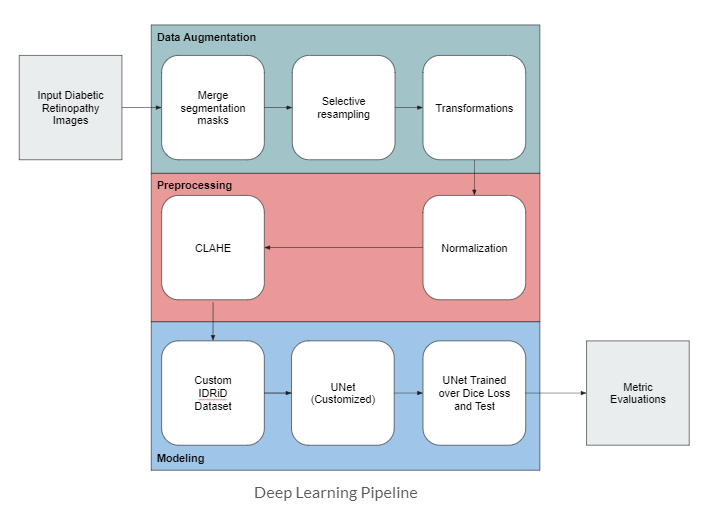
\includegraphics[scale=0.7]{image/dl_pipeline.PNG}
	\caption{Deep Learning Pipeline Overview}
	\label{fig:dl}
\end{figure*}

\subsubsection{Data Description}
\label{sssec:describe}
We have a total of 54 train images and 27 test images which is a multi class segmentation problem. 
\par
The input images contains the 3 channel retina and the label images contain 4 images of 1 channel diabetic lesions namely Microaneurysms, Haemorrhages, Hard Exudates and Soft Exudates per every input image.

\subsubsection{Merge Segmentation masks}
\label{sssec:merge}

A single segmentation mask was generated from the available segmentation masks per image by stacking binary masks across an axis and taking the argmax per pixel. This resulted in integer encoding of the 4 categories of the lesions and the background.
\begin{itemize}
		\item \textbf{0} Background
		\item \textbf{1} Haemorrhages
		\item \textbf{2} Hard exudates
		\item \textbf{3} Microaneurysms 
  		\item \textbf{4} Soft Exudates
\end{itemize} 

\subsection{Data Preprocessing}
\label{ssec:preprocess}
Incomplete and noisy data are common properties of real world databases. Data needs to be cleaned before it is processed for better efficiency and accurate outputs. There are a lot of pre-processing techniques that include cleaning and preparing the data for classification. Other pre-processing techniques include Integration and Transformation, Aggregation and Discretization.

The pre-processing done for our data are,
\begin{itemize}
\item \textbf{\textit{Filling missing values}} Missing values are filled in many ways and we used the mean of the total and substituted with our missing values. 
\item \textbf{\textit{Removal of unnecessary attributes}} Unnecessary attributes are removed so that it doesn't affect the performance of the model.
\item \textbf{\textit{Encoding the attribute values}} The values in the label \textit{sex} are in the form of characters \textit{M/F} which are transformed to \textit{1/0} using the help of label encoder.
\end{itemize} 

\subsection{Feature Selection}
\label{ssec:featureselect}
Selecting the right features for classification is very important and it  is the key factor for achieving a good performance for a model. 
\par
The models are having a very high deviation due to the presence of the \textit{id} label because of its sequence ordering nature. So, the \textit{id} label gets high feature importance, but, it is just a patient identifier which should be dropped from the data-set. The remaining labels are all important to process the output label. So the remaining 8 labels with 1384 patients are taken for classification. 
\subsection{Feature Scaling}
\label{ssec:featurescale}
Feature Scaling is important when the bounds between the labels are different from each other. The upper and lower bounds of the labels are very important and if they vary a lot in the data-set that could affect the performance of the model. There are many feature scaling techniques like standard scalar which makes use of mean and standard deviation, min-max scalar which normalizes based on the minimum and maximum values and robust scalar which makes use of the quartile ranges to normalize.
\par 
We used standard scalar as it fits the data based on the mean and the deviation of the data. Standard scalar is given by 
\begin{equation}
 y_{Scaling} = \sum\limits_{i=1}^{n}\frac{x_i - \mu(x) }{\sigma(x)}
\end{equation}
where n is the number of patients, $\mu(x)$ is the mean and 
$\sigma(x)$ is the standard deviation for the label.
\subsection{Classification}
\label{ssec:classification}
Classification is a 2-step process. In first step, a classifier is built to describe a predetermined set of data classes. This is the learning step and is done using the training data, where a classification algorithm builds the classifier by learning from that training set made up of data tuples and their associated class labels. It is also known as “Supervised learning”. 
\par
The data-set consists of 1384 patient details of which 80\% are taken for training the data and the remaining 20\% are taken for testing the data. The following are the learning algorithms that we used to predict the output label \textit{death},
\begin{enumerate}
\item Support Vector Machine
\item Linear Discriminant Analysis
\item Logistic Regression
\item Decision Tree Classifier
\item Naive Bayes
\item Random Forest Classifier
\item K - Nearest Neighbor
\end{enumerate}
\par
\subsubsection*{Support Vector Machine}
Support Vector Machines(SVM) are the supervised learning models that are used for classification of the data. SVMs are designed for both linear as well as non-linear classification. Linear data is rare and most of the existing data is non-linear. So, in \cite{svm}, they designed the SVM to fit the non-linear data by using the kernel trick which uses kernels in SVM to fit the data accordingly. There are many kernels that can be used on a data. As it is a hyper-parameter we need to experiment it with all the available kernels to find the best fit.
\begin{table}[ht]
\centering
 \begin{tabular}{|c| c c|} 
 \hline
 Kernel  & \thead{Train \\ Accuracy} & \thead{Test \\ Accuracy} \\ [0.5ex] 
 \hline
 Linear Function & 0.779 & 0.815\\ 

 Polynomial Function & 0.783 & 0.779\\
 
 Radial Basis Function & 0.807 & 0.826\\
 \hline
\end{tabular}
\vspace*{0.25cm}
\caption{SVM Kernels and their accuracies}
\label{table:svm}
\end{table}
\par
The following kernels and its accuracies that are used for our data are listed in the Table \ref{table:svm}. As we can see Radial Basis Function(RBF) kernel fits the data better than other experimented kernels because it has proved to be a generalizer for many data-sets and in many experiments it is assumed as priors for uncertain situations. RBF is also called squared exponential kernel or gaussian kernel.            


\subsubsection*{Decision Tree Classifier}
Decision tree is a, supervised learning algorithm, which is widely used classifier. Unlike Naïve Bayes, Logistic regression and other algorithms that belong to the supervised learning algorithm family, it can be used for solving both regression and classification problems. Even when the dataset has missing values, using Decision tree could result in a better output.
\par

When applied directly, Decision Tree causes the overfitting on \cite{monoclonal1} and not being generalized well to the new data. Therefore we pre-pruned the tree by setting the maximum depth $max_{depth}$ parameter to 3 as seen from \cite{dt}. Thus decreasing overfitting by limiting the depth. We observed a decrease in accuracy on the training set, but a significant increase in accuracy of test data. The feature importance plot of the decision tree classifier as shown in the figure \ref{feature_dtc} is given by,
%
%\begin{figure}[h!]
%	\centering
%	\includegraphics[width=3.5in]{../Images/images/feature_dtc.png}
%	\caption{Feature Importance plot of Decision Tree Classifier}	
%	\label{feature_dtc}
%\end{figure}
Information Gain and Gini Index are the two attribute selection measures used for selecting which attribute can be considered as the root node at each level. Figure \ref{gini} shows use the visualization of how gini index acts on the data-set.

%%Addition of the data
%\begin{figure*}[h!]
%	\centering
%	\includegraphics[scale=0.4]{../Images/dtree2.png}
%	\caption{Visualization of Decision Tree Classifier using the gini index selection measure}	
%	\label{gini}
%\end{figure*}

\subsubsection*{Naive Bayes}
Naive Bayes, a highly scalable algorithm which is a special case of Bayesian Network where it is assumed that all the features are independent given the class label. Presence or absence of one feature will not influence the presence or absence of other features. Given a class label $C$, the relationship between conditionally independent data $x_i$ can be given by the formula,
%\begin{figure}[H]
%	\centering
%	\includegraphics[width=3.5in]{../Images/images/nb.png}
%	\label{fig:nb}
%\end{figure}
%Formula
\par
The algorithm predicts the class of a previously unseen test case $X={x_1, x_2... x_n}$ by choosing the class that maximizes the above equation. In practice the predictor prior probability p(x) can be omitted because the classification focuses on choosing the class that maximizes the equation. From \cite{nb} we can say that, one of the advantages of the NB classifier is that it requires only few amounts of training data to estimate the class variables needed for classification. It is one of the popular choices for text classification, binary and multi-class classification problems.

\subsubsection*{Random Forest Classifier}
Random Forest, similar to Decision Tree Classifier can be used for solving both regression and classification problems. It is an ensemble learning model. \cite{rf}  The algorithm creates forest with a number of Decision Trees. More the trees in the forest, higher the accuracy of the classifier. 
\par

The algorithms gives importance to certain features to make a prediction. Not all the attributes are considered equal and thus the result vary for different data-sets. The randomness in building the random forest forces the algorithm to consider many possible explanations. Thus result of random forest captures a much broader picture of the data than a single tree. The feature Importance plot of the random forest classifier in figure \ref{rfc}, is given by, 
%
%\begin{figure}[ht!]
%	\centering
%	\includegraphics[width=3.5in]{../Images/images/feature_rfc.png}
%    \caption{Feature Importance plot of Random Forest Classifier}	
%	\label{rfc}
%\end{figure}
\par
\begin{itemize}
\item In this algorithm, \textbf{k} features are randomly selected from a total of \textbf{n} features.
\item Among the \textbf{k} features, using the best split point node \textbf{d} is calculated.
\item The node is now split into daughter nodes using the best split.
\item The above 3 steps are iterated until \textbf{l} number of nodes are formed.
\end{itemize}
Repeat the above 4 steps \textbf{m} times until \textbf{m} decision trees are formed. Two important features of RF are: 
\begin{enumerate}
\item Ability to achieve high prediction accuracy.
\item Usability of desired capabilities.
\end{enumerate}


\subsubsection*{K - Nearest Neighbor}
K Nearest neighbors is a classification algorithm that is used for regression predictive problems. As seen from \cite{knn}, building the model will only store the training data set. Only if a new input is chosen, it predicts and finds the closest data points in the training data: \textit{nearest neighbor}. KNN is commonly used for its easy of interpretation and minimal calculation time.
\par
The figure below shows the training and test data accuracy on the y-axis against number of neighbors on the x-axis. Consider choosing one single nearest neighbor, accuracy of prediction on training data set is \textbf{1}, perfect. But if more neighbors are considered, the training accuracy falls, showing us that using the single nearest neighbor leads to a model that is much complex.


%Figure of KNN
%\begin{figure}[h!]
%	\centering
%	\includegraphics[width=3.5in]{../Images/images/knn1.png}
%	\caption{Accuracies of KNN on train and test data}
%	\label{fig:knn}
%\end{figure}
\par
Figure \ref{fig:knn} indicates us to choose 17 or 18 neighbors. In our case K=17 neighbors has produced an accuracy of 81.2\% while K=13 neighbors has produced an accuracy of 82.3\%.


Thus we know how much the choice of factor \textbf{K} in the algorithm influences the outcome. The boundary becomes smoother with the increasing value of \textbf{K}. The training accuracy and test accuracy are the two parameters needed to access on different K-value, as shown the plot figure. The accuracy of KNN classifier significantly increases by increasing the number of data rows in the training set.


\subsection{Metrics}
\label{sec:metrics}
The combination of all the steps are evaluated under different performance metrics, including accuracy, accuracy per class, Jaccard Similarity Coefficient, Dice Similarity Coefficient for the multi class Segmentation. The metrics are defined as following,

\begin{equation}
JSC = \frac{|S \cap T|}{|S \cup T|} = \frac{|TP|}{|TP| + |FP| + |FN|}
\end{equation}

\begin{equation}
DSC = 2\frac{|S \cap T|}{|S| + |T|} = \frac{2|TP|}{2|TP| + |FP| + |FN|}
\end{equation}

\begin{equation}
Accuracy = \frac{1}{n}\sum\limits_{i=1}^{n} \frac{|X_i \cap Y_i|}{|X_i \cup Y_i|}
\end{equation}

where $TP$ is the true positive, $FP$ is the False Positive, $FN$ is the False Negative, $X_i$ is the set of predicted labels, $Y_i$ is the set of true labels and n is the number of samples.

\section{Results and Analysis}
Table \ref{table:1} shows us the model performance for all the algorithms we have experimented. The metrics used for evaluation are accuracy, precision, recall and $F_1$-score as shown in the section \ref{sec:metrics}. As we can see, the comparison between the algorithms helped us understand the nature of the algorithm as well as the data used, based on the metrics. The accuracies of all the other algorithms are close to each other by a fraction of percentage as they are tweaked to get the best accuracy using kernels, solvers and hyper-parameters. Except Naive Bayes all the accuracies of other algorithms are above 80\%. 
\par
The highest accuracy was achieved by Support Vector Machine with the radial basis function as the kernel. Its accuracy is 82.6\%. Therefore, the data is non-linear and it takes the form of probabilistic density function which has a global maximum. The lowest accuracy is achieved by Gaussian Naive Bayes but the difference in accuracies between the highest and lowest is only 2.9\%. When we consider the data to be linear, the accuracy falls below 60\%. Finally, the overall precision, recall and $F_1$-score for the algorithms are similar for many cases with the highest achieved by Support Vector Machine.
\par

\begin{table}[H]
\centering
 \begin{tabular}{|c| c c|} 
 \hline
 Metrics & Train & Test\\ [0.5ex] 
 \hline
 Overall Accuracy & 0.9460 & 0.9272\\ 
 \hline
 Accuracy per class & 0.4570 & 0.4130\\
 \hline
 Jaccard Similarity & 0.3431 & 0.3093\\
 \hline
 Dice Similarity & 0.4253 & 0.3838\\
 \hline
\end{tabular}
\vspace*{0.25cm}
\caption{Model Performance of UNet}
\label{table:1}
\end{table}

Table \ref{table:2} gives the performance measure for the output labels whose deaths is classified as \textbf{0}. As we can see, the values of the metrics, precision, recall and $F_1$-score are very less when compared to the metrics in table \ref{table:3}. That is because the number of patient with the output label \textbf{0} are very less when compared to the number of patients with output labels \textbf{1}. As the  $F_1$-score is a harmonic mean of precision and recall we can a reasonable values for it unlike the other two. The highest precision, recall and $F_1$-score is achieved by Random Forest Classifier, Decision Tree Classifier respectively. 
\begin{table}[H]
\centering
 \begin{tabular}{|c| c c c|} 
 \hline
 Techniques  & Precision & Recall & F1-score \\ [0.5ex] 
 \hline
 Support Vector Machine & 0.81 & 0.59 & 0.68 \\ 
 \hline
 Linear Discriminant Analysis & 0.77 & 0.60 & 0.68\\
 \hline
 Logistic Regression & 0.79 & 0.59 & 0.68\\
 \hline
 K - Nearest Neighbor & 0.77 & 0.64 & 0.70\\
 \hline
 Naive Bayes & 0.66 & 0.75 & 0.70\\  
 \hline
 Decision Tree Classifier & 0.72 & 0.69 & 0.71 \\
 \hline
 Random Forest Classifier & 0.82 & 0.51 & 0.63  \\[0.75ex] 
 \hline
\end{tabular}
\vspace*{0.25cm}
\caption{Performance Measures of the prediction when deaths label value is \textbf{0}}
\label{table:2}
\end{table}


The performance measures for prediction when the output labels is \textbf{1} is very high because of the dominance of the binary value \textbf{1} in the data. From Table \ref{table:3}, we can see that the highest precision, recall and $F_1$-score is achieved by Decision Tree Classifier, Support Vector Machines respectively. 
\begin{table}[H]
\centering
 \begin{tabular}{|c| c c c|} 
 \hline
 Techniques  & Precision & Recall & F1-score \\ [0.5ex] 
 \hline
 Support Vector Machine & 0.83 & 0.94 & 0.88 \\ 
 \hline
 Linear Discriminant Analysis & 0.83 & 0.92 & 0.87\\
 \hline
 Logistic Regression & 0.83 & 0.93 & 0.87\\
 \hline
 K - Nearest Neighbor & 0.84 & 0.91 & 0.88\\
 \hline
 Naive Bayes & 0.88 & 0.82 & 0.85\\  
 \hline
 Decision Tree Classifier & 0.86 & 0.87 & 0.87 \\
 \hline
 Random Forest Classifier & 0.81 & 0.95 & 0.87  \\[0.75ex] 
 \hline
\end{tabular}
\vspace*{0.25cm}
\caption{Performance Measures of the prediction when deaths label value is \textbf{1}}
\label{table:3}
\end{table}


\section{Conclusion and Future Work}
\subsection{Task 1}
In this paper, the problem of summarizing UNet Deep Learning model which is used for retinal lesions associated with Diabetic Retinopathy in Augmented IDRiD datasets is discussed. The focus is mainly on using customized UNet to effectively segment the retinal lesions associzted with Diabetic Retinopathy \cite{monoclonal1} . For prediction we used an augmented dataset with 940 train images and 236 validation images and it is preprocessed to remove noise and contrasted with CLAHE. The outcome of the predictive results on the IDRiD data-set reveals the accuracy, accuracy per class, Jaccard Similarity Coefficient and Dice Similarity Coefficient with a score of 92.72, 41.30, 30.93, 38.38 \% respectively. The second conclusion gives us an intuition of how Dice loss performed better than the other loss functions like Binary cross entropy without weights, pixel wise cross entropy using weights.
\par 
The proposed work can be enhanced by expanding its scope to using Transfer Learning with pre trained models like Resnet 50, Resnet 101 or Inception v3. Hyper parameter Tuning the weights for the data imbalance will also improve the Pixel wise Cross Entropy Loss Function and finally we can use different type of Segmentation models like Residual nets, FCN etc.,

\subsection{Task 2}
In this paper, the problem of summarizing different algorithms of Machine Learning used for the prediction of deaths due to Monoclonal Gammopathy is discussed. The focus is mainly on using different algorithms to effectively predict the deaths due to MGUS \cite{monoclonal1} . For prediction we used a refined version of the data-set with 9 attributes that are produced after applying a few data mining techniques. The outcome of the predictive results on the same data-set reveals that Support Vector Machine has outperformed all the other algorithms in terms   of accuracy, precision, recall and $F_1$-score with a score of 82.6, 83, 83, 82 \% respectively. The second conclusion gives us an intuition of how the output labels affect the metrics, by analyzing it in detail on the output labels.
\par 
The proposed work can be enhanced by expanding its scope to using Transfer Learning prediction by using  the deep learning techniques \cite{dl,dl2}  like Artificial  Deep Neural Networks, Multi-perceptron etc.,
which have been proven to have increased the performance of many data-sets due to its nature of deep computation.

\bibliographystyle{IEEEtran}
\bibliography{references}




% that's all folks
\end{document}


